\chapter{Módulo Servidor}
\noindent
Este capítulo tem o objetivo de abordar o 1º módulo desenvolvido para atender o objetivo proposto, o módulo do servidor. De maneira geral, como já mencionado, ele é o responsável por analisar a fotografia da turma, assim como os dados pertinentes. Ele deverá detectar as faces na fotografia e depois, utilizando o algoritmo LBPH, identificar cada uma delas. Para cada face reconhecida deve-se atribuir a presença, a qual será enviada para o armazenamento persistente, o banco de dados PostgreSQL. Ele está relacionado aos requisitos funcionais \textit{RF01 - Apurar falta} e   \textit{RF04 - Armazenar fotografia}. Ele atende ao caso de uso \textit{UC-01 Apurar falta}. Optou-se por abordar o processo de envio e recebimento das fotografias e dados, no módulo \textit{mobile}. Assim a atividade do módulo servidor se inicia ao detectar uma fotografia na pasta faltas.  

\section{Conceito Geral do módulo}
\noindent
 Segundo \citep{Arubas} o reconhecimento compara a face (desconhecida) que se quer reconhecer com um conjunto de treinamento de faces conhecidas. No conjunto de treinamento, são fornecidas as faces e a qual pessoa elas pertencem. Quando é solicitado ao algoritmo que reconheça alguma face desconhecida, ele usa o conjunto de treinamento para fazer o reconhecimento. Ele destaca ainda que, o LBPH analisa cada rosto no conjunto de treinamento de forma individual e independente. 
 
O presente projeto utilizou a biblioteca OpenCV, onde se explorou os algoritmos \textit{HaarCascade}, detecção de olhos e o de detecção de faces, para a detecção com maior grau de certeza das faces e o LBPH para o reconhecimento da face. O OpenCV, conforme \citep{opengeral2018}, é uma biblioteca gratuita para uso no meio acadêmico e comercial. Ela é voltada para visão computacional e aprendizado de máquina, tendo sido escrita primeiramente em C++. Possui interfaces nas linguagens C++, Python, Java e MATLAB.

Optou-se por utilizar a interface na linguagem Python, devido as características da linguagem, tais como facilidade de leitura e compreensão, além da fácil manutenção. Nesse sentido, \citep{pythonLTC} diz que Python é uma linguagem caracterizada como sendo de uso geral, que foi idealizada para fazer com que os programas sejam muito legíveis, isso é, priorizou-se a legibilidade. Além disso, Python também possui inúmeras  bibliotecas,  isso torna possível a escrita de aplicações sofisticadas, mas com aparência simples. Pelas razões apresentadas, o mencionado autor conclui que "Python tornou-se uma linguagem de desenvolvimento de aplicações popular e também uma preferência como “primeira” linguagem de programação"\ \cite[p. 22]{pythonLTC}. 

Vale destacar nesse momento uma particularidade do Python. Conforme \citep{pythonLTC}, a versão 2 não é compatível com a  3. Isso significa que um programa escrito em Python 2, provavelmente, não irá funcionar usando um interpretador de Python 3. \citep{pythonLTC} considera que a versão 3 apresenta uma maior consistência que a 2. Nesse aspecto, optou-se por utilizar o Python 3.6.3, o qual foi, segundo \citep{python_org}, lançado em 03 de outubro de 2017. 
 
Quanto ao OpenCV, a versão escolhida foi a 3.4.2. Essas considerações sobre as versões se justificam devido ao fato de que por vezes, métodos e formas de trabalho idealizadas para uma determinada versão, acabam sendo modificados em versões seguintes. Justamente para evitar esse tipo de problema, optou-se por utilizar uma única versão ao longo do desenvolvimento do trabalho.
 
 
\section{Etapas pré-reconhecimento}
\noindent 
Antes de realizar o reconhecimento facial, faz-se necessário realizar o treinamento, isso é, gerar o conhecimento sobre a turma, gera-se um arquivo que concatene as informações extraídas de cada uma das fotografias, mantendo a identificação (a quem pertence) de cada uma das faces aprendidas. Para isso, segue-se as seguintes etapas ilustradas na figura \ref{fig:figura50}

\begin{figure}[!ht]
	\centering
	
\includegraphics[width=1\textwidth]{UML_cap_mod1.png}   
	\caption{Diagrama de atividades da fase pré-reconhecimento}
	\label{fig:figura50}
\end{figure}

Na primeira etapa deve-se fotografar o aluno de forma individual, com uma grande variedade de expressões, ângulos de fotografia e incidência de luz. Essa é uma etapa muito importante, pois essas imagens formarão a base de conhecimento (imagens a serem treinadas). 

Depois disso, utiliza-se o artefato responsável pela conversão, desenvolvido ao longo do módulo servidor. Ele faz com que a fotografia seja transformada em uma escala cinza, ocorra a detecção da face utilizando o \textit{haarcascade frontal face}, depois disso, essa região é verificada com o \textit{haarcascade eye}, a fim de eliminar-se resultados falso-positivos, isso é, eliminar a situação em que um objeto é reconhecido erroneamente como uma face. Por fim ocorre o recorte dessa face já na escala cinza e em um mesmo tamanho (720x720). Nesse ponto vale destacar que não são todas as fotografias que irão gerar faces válidas, uma vez que o \textit{haarcascade frontal face} e o \textit{haarcascade eye} podem não detectar nenhuma face, mesmo havendo. O programa recebe do usuário o nome da turma, e converte todas imagens contidas na pasta com esse nome. Oferece ainda ao usuário a opção de escolher se deseja exibir cada uma das fotografias antes da converter ou não. Ao final da conversão das imagens de cada aluno, exibe-se a quantidade de imagens lidas, e a quantidade de faces reconhecidas, isso é, que foram de fato aproveitadas e geraram uma nova imagem. A figura \ref{fig:figura51} ilustra esse procedimento, mostrando além do nome do arquivo, sua luminosidade. 

\begin{figure}[!ht]
	\centering
	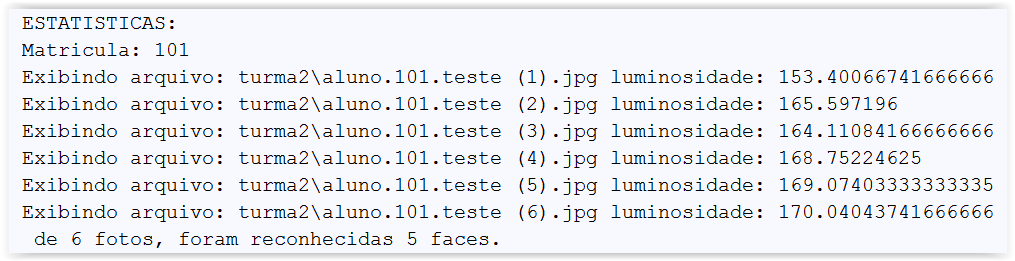
\includegraphics[width=0.9\textwidth]{conversor_saida_estatistica.PNG}   
	\caption{Informações estatísticas exibidas ao final do processo conversor}
	\label{fig:figura51}
\end{figure}

Uma padronização adotada foi o nome dado às fotografias, optou-se por utilizar a seguinte concatenação de nomes "aluno" + "." + o número da matrícula do aluno + "." + nome da turma + " (" + número da fotografia + ").jpg", por exemplo: "aluno.101.comp18 (1).jpg", na figura \ref{fig:figura51} o nome  de turma usado foi "teste". Essa padronização de nomenclatura facilita o processo de codificação e foi utilizada para armazenar o número da foto e a matrícula do aluno. As imagens de alunos de uma mesma turma foram agrupadas em uma mesma pasta. A figura \ref{fig:figura52} ilustra um exemplo de entrada e saída do procedimento descrito acima. Ao final dessa etapa, tem-se as imagens já convertidas, redimensionadas e recortadas. 

\begin{figure}[!ht]
	\centering
	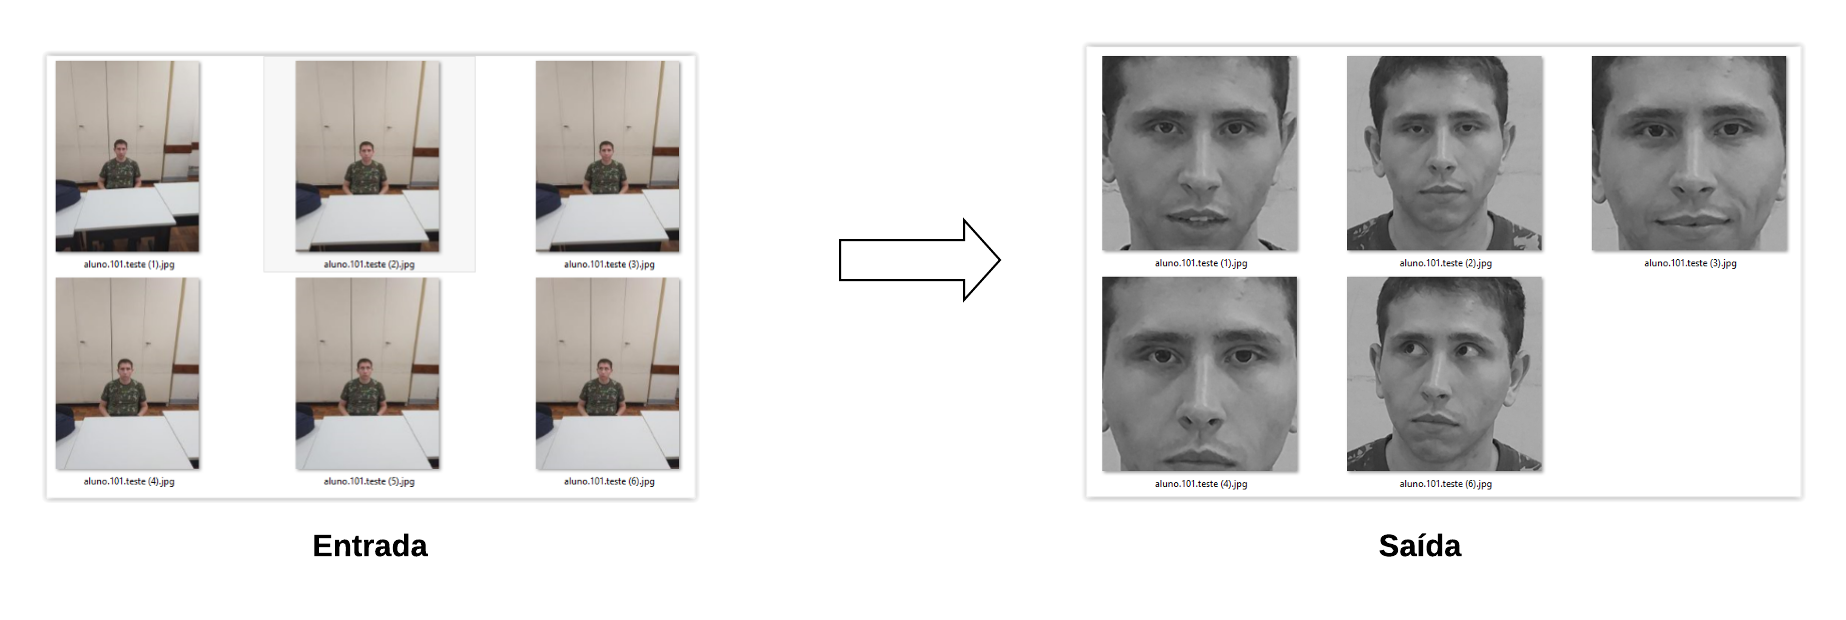
\includegraphics[width=1.0\textwidth]{entrada-conversor-saida.png}   
	\caption{Entrada e saída do conversor}
	\label{fig:figura52}
\end{figure}


\subsection{O treinamento e seus parâmetros}
\noindent
Na etapa seguinte gera-se o arquivo com as informações extraídas das faces, usando-se a metodologia do LBPH, anteriormente apresentada. Assim, através do artefato, desenvolvido ao longo do módulo servidor, "criador\_de\_inteligencia"\ irá se gerar o arquivo de treinamento. Esse é o primeiro momento que o algoritmo LBPH é de fato empregado. Ao se invocar o método \textit{LBPHFaceRecognizer\_create}, tem-se de escolher alguns valores para determinados parâmetros. Quando explicou-se sobre o algoritmo LBPH, eles foram detalhados. São eles:
\textit{radius, neighbors, grid\_x, grid\_y, threshold} 

O parâmetro \textit{radius}, segundo \citep{openlbph2018}, consiste no raio usado para construir o Padrão Binário Local Circular. Raios maiores, tornam mais suaves as imagens, porém, carregam mais informações espaciais. 

Para o parâmetro \textit{neighbors}, \citep{openlbph2018} explica que quanto maior o valor usado para a quantidade de vizinhos, maior será o gasto computacional, ela sugere o uso do valor 8. Esse valor corresponde a uma matriz 3X3, onde pode-se pensar no elemento central, isso é, elemento na linha 2 e coluna 2, como sendo o elemento a ser analisado. Os demais elementos dessa matriz, seriam os vizinhos utilizados. 

Já para o parâmetro \textit{grid\_x} e \textit{grid\_y}, número de células na horizontal e vertical respectivamente, apesar de \citep{openlbph2018} explicar que muitas publicações sugerem o uso do valor 8, os testes realizados no presente projeto obtiveram melhores resultados com o valor 12.

Para melhor escolher os valores a serem utilizados para \textit{neighbors}, \textit{grid\_x} e \textit{grid\_y} realizou-se alguns testes. Utilizou-se o banco de imagens disponibilizado pela Universidade de Yale. \citep{yales} explica que esse banco contém 165 imagens em escala cinza, de 15 pessoas diferentes, havendo portanto 11 imagens por pessoa. Essas imagens variam as expressões da face e condições de iluminação. Além disso, \citep{yales} esclarece que o banco de imagens está disponível publicamente para uso que não seja comercial. As imagens foram convertidas para o formato jpg, por questões de compatibilidade com a biblioteca OpenCV. Os testes consistiram em variando os parâmetros \textit{neighbors}, \textit{grid\_x} e \textit{grid\_y} verificar o índice de acerto no reconhecimento facial. 

Sobre os testes, foram escolhidas 2 imagens de cada pessoa para serem reconhecidas, o que totaliza 30 fotografias. As imagens restantes, isso é, 9 imagens por pessoa, foram utilizadas no treinamento. Como saída do teste, obteve-se a Tabela \ref{tab:tabela1}, nela X e Y referem-se respectivamente aos valores utilizados em \textit{grid\_x} e \textit{grid\_y},  a coluna acertos é exibida em percentagem, já tamanho refere-se ao arquivo gerado pelo treinamento em megabytes, tempo 1 e tempo 2 foram obtidos em segundos e referem-se ao gasto no treinamento, e o total nos reconhecimentos, respectivamente. Por fim  distância refere-se ao somatório das distâncias entre as imagens em análise (faces a serem reconhecidas) e as imagens que mais se aproximam delas. Vale destacar, que em virtude da apuração de tempo, os testes foram repetidos 5 vezes e o tempo mostrado trata-se de uma média aritmética.

Nesses testes, adotou-se o parâmetro \textit{threshold}, no valor de 1000, nos próximos parágrafos serão feitos mais comentários sobre isso. O que vale destacar é que esse valor extremamente alto, força com que a face em análise seja reconhecida como uma das pessoas cadastradas no treinamento.        


% ii. tabelas: usar \begin{sidewaystable} ... \end{sidewaystable}
%                    em vez de \begin{table} ... \end{table}

\begin{table}[ht]
\centering
\caption{Testes com os parâmetros do método \textit{LBPHFaceRecognizer\_create}.}
\vspace{0.5cm}
\begin{tabular}{ccccccccc}
 
Radius & Neighbors & X & Y & Acertos & Tamanho & Tempo 1 & Tempo 2 & Distância \\
\hline
1 & 4 &8 &8 &66.66\% & 2.1 & 1.73 &2.01 & 3.25 \\
1 & 5 &8 &8 &66.66\% & 3.9 & 1.64 &2.17 & 4.45 \\
1 & 6 &8 &8 &66.66\% & 6.6 & 2.63 &2.38 & 6.9 \\
1 & 7 &8 &8 &63.33\% & 10.8 & 2.83 &2.76 & 6.8 \\
1 & 8 &4 &4 &63.33\% & 6.08 & 2.72 &2.5 & 0.9 \\
1 & 8 &6 &6 &63.33\% & 11.6 & 3.44 &2.85 & 3.39 \\
1 & 8 &8 &8 &66.66\% & 18.5 & 5.27 &3.44 & 10.69 \\
1 & 8 &10 &10 &66.66\% & 26.7 & 5.72 &4.15 & 21.53 \\
1 & 8 &12 &12 &70\% & 36.3 & 7.30 &5.10 & 38.00 \\
1 & 8 &14 &14 &70\% & 47.0 & 8.36 &6.09 & 62.61 \\
1 & 9 &12 &12 &70\% & 60.1 & 10.32 &7.32 & 40.79 \\
1 & 9 &14 &14 &70\% & 79.3 & 11.62 &8.69 & 65.87 \\
2 & 8 &8 &8 &63.33\% & 20.4 & 4.20 &3.49 & 11.72 \\
2 & 10 &10 &10 &60\% & 82.8 & 13.72 &8.95 & 30.55 \\
3 & 8 &8 &8 &60\% & 21.3 & 5.46 &3.50 & 12.32 \\

\end{tabular}
\label{tab:tabela1}
\end{table}

A partir da Tabela \ref{tab:tabela1}, concluiu-se pela escolha dos parâmetros da seguinte forma: \textit{radius = 1, neighbors = 8, grid\_x = 12, grid\_y = 12}. Essa escolha se deu, pois foi o conjunto de parâmetros que obteve a maior taxa de acerto, combinada com um menor somatório de distância.

Por fim, o parâmetro \textit{threshold}, é um dos mais importantes e de difícil escolha. Tem-se que uma situação comum no reconhecimento facial é dizer se uma determinada face pertence ao conjunto de treinamento ou se é desconhecida. O parâmetro \textit{threshold}  refere-se ao limite, no teste cujo resultado foi mostrado acima, o algoritmo calcula a distância entre a face em análise e as que foram treinadas. O menor valor de distância encontrado é comparado com o \textit{threshold}, se o primeiro for maior que o segundo a face em análise será classificada como desconhecida, caso contrário é atribuída ao elemento ao qual pertence a face de treinamento com menor distância.

No caso de uma turma de aula, todas as faces, que aparecem na fotografia tirada no início do tempo de aula, pertencem a um aluno regularmente matriculado. Em outras palavras, não existe a situação de uma face não pertencer a alguém que não esteja no conjunto de treinamento. Essa afirmação poderia levar a falsa ideia de que a solução seria colocar um valor extremamente elevado para o parâmetro \textit{threshold} forçando o algoritmo a não classificar uma face como desconhecida. Percebeu-se em alguns casos, como na figura \ref{fig:figura53}, que dado um aluno X, pode acontecer que na fotografia da turma (aquela a se apurar a falta), sua face fique distante das faces previamente utilizadas para a geração do conhecimento (treinamento) da turma. Ao se utilizar o parâmetro \textit{threshold} elevado, o algoritmo acabou por classificar aquele aluno X, como sendo outro aluno, o que mais se aproxima, mesmo esse não sendo o aluno X. A figura \ref{fig:figura53} ilustra um exemplo em que isso aconteceria. Colocando um parâmetro de \textit{threshold} elevado, a face em análise seria reconhecida como sendo a correspondente ao Aluno B, o que seria uma classificação errada. 

\begin{figure}[!ht]
	\centering
	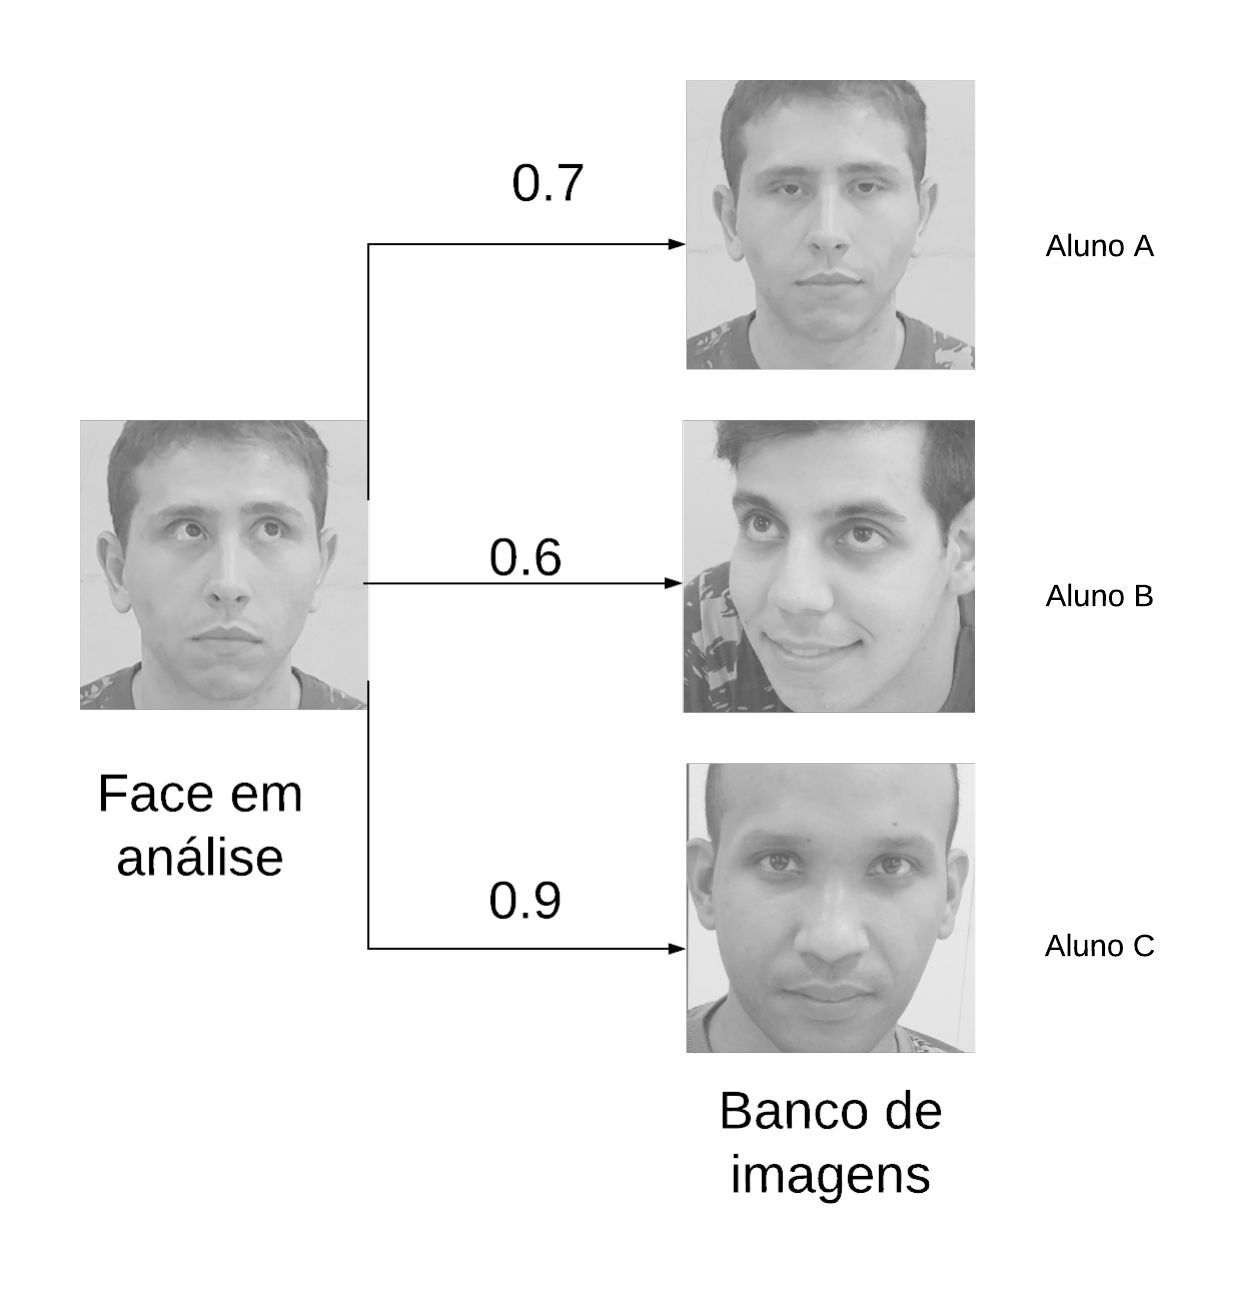
\includegraphics[width=0.6\textwidth]{threa.png}   
	\caption{Exemplo de distância menor que o limite, gerando classificação incorreta }
	\label{fig:figura53}
\end{figure}


A dificuldade na escolha desse parâmetro está no fato de quando é melhor classificar a face como desconhecida ao invés de tentar forçar uma classificação com distância maior, e que pode ser errada. Ao utilizar um valor elevado, pode-se forçar classificações erradas. Por outro lado, colocar valores baixos pode fazer com que se classifique uma face como desconhecida enquanto que ela poderia utilizar a classificação que lhe seria dada dentre o conjunto. Pensando no caso da figura \ref{fig:figura54}, caso fosse adotado um \textit{threshold} de 0.5, a análise concluiria que a face pertence a um elemento desconhecido. Por outro lado um \textit{threshold} de 0.7 seria suficiente para uma classificação correta.

\begin{figure}[!ht]
	\centering
	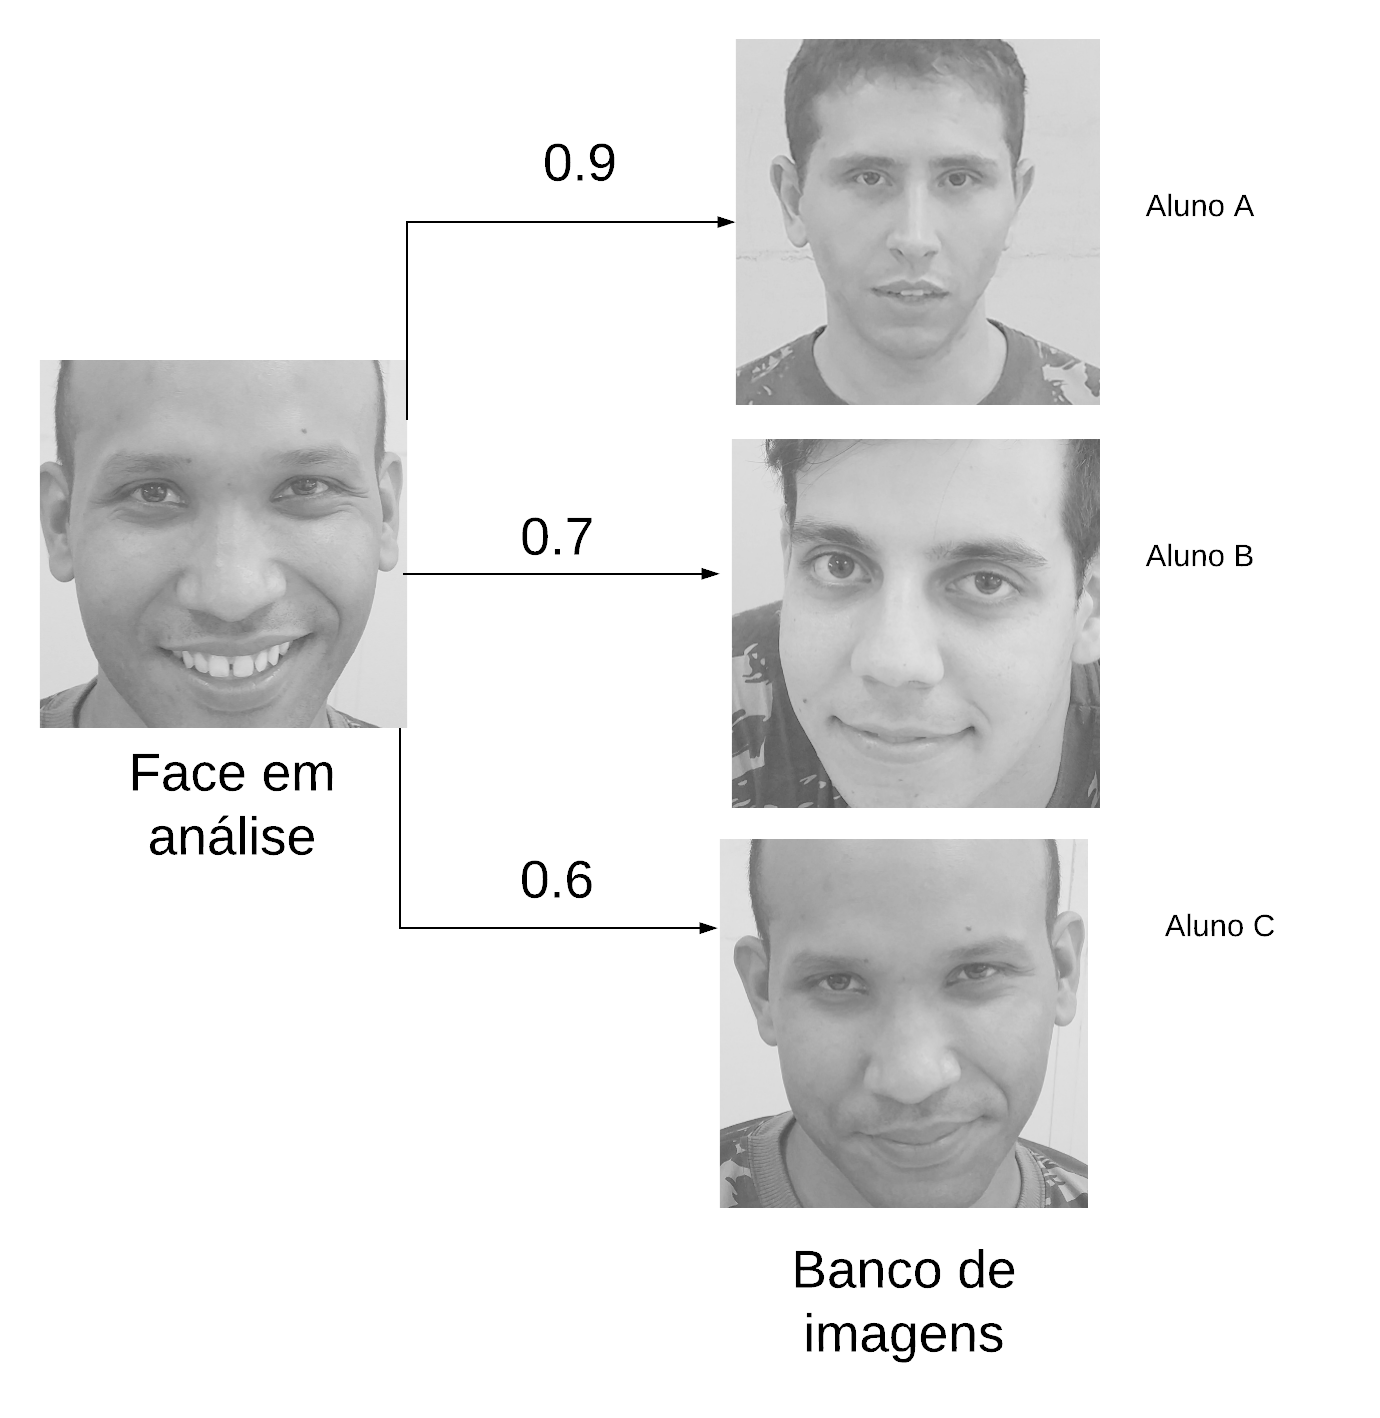
\includegraphics[width=0.6\textwidth]{threb.png}   
	\caption{Exemplo de distância maior que o limite, gerando classificação desconhecida }
	\label{fig:figura54}
\end{figure}

%Como saída do teste, obteve-se a Tabela \ref{tab:tabela1}, 
Feitas as considerações acima, realizou-se o procedimento similar ao descrito no início da subseção, isso é, utilizou-se o banco de imagens  disponibilizado pela Universidade de Yale \citep{yales}, contendo 165 imagens, dais quais 30 foram utilizadas para serem reconhecidas e as outras 135 para a geração do arquivo de treinamento. Ao gerar o arquivo de treinamento, utilizou-se como parâmetro os  encontrados anteriormente, \textit{radius = 1, neighbors = 8, grid\_x = 12, grid\_y = 12}. A Tabela \ref{tab:tabela2}, traz o valor de \textit{threshold}, a quantidade de faces detectadas com acerto, classificadas como desconhecidas e erradas. As quantidades estão em valores absolutos. Perceba que a classificação como desconhecida não é considerada como um erro, nem como um acerto. Em cada linha da tabela, a soma de acerto, desconhecida e erro totaliza 30, que é o número de imagens testadas.

% ii. tabelas: usar \begin{sidewaystable} ... \end{sidewaystable}
%                    em vez de \begin{table} ... \end{table}

\begin{table}[ht]
\centering
\caption{Testes para determinação do \textit{threshold}.}
\vspace{0.5cm}
\begin{tabular}{cccc}
 
threshold & Acerto & Desconhecida & Erro \\
\hline
10	& 3	& 27	& 0   \\
15	& 3	& 27	& 0  \\
20	& 3	& 27	& 0  \\
25	& 6	& 24	& 0  \\
30	& 7	& 23	& 0  \\
35	& 8	& 22	& 0  \\  
40	& 13	& 17	& 0  \\
45	& 17	& 13	& 0  \\
50	& 18	& 12	& 0  \\
55	& 18	& 12	& 0  \\
60	& 18	& 12	& 0  \\
65	& 18	& 11	& 1  \\
70	& 18	& 11	& 1  \\  
75	& 19	& 10	& 1  \\
80	& 19	& 9	& 2  \\
85	& 20	& 7	& 3  \\
90	& 20	& 5	& 5  \\
95	& 20	& 4	& 6  \\
100	& 20	& 3	& 7  \\
110	& 20	& 2	& 8  \\
130	& 21	& 0	& 9  \\


\end{tabular}
\label{tab:tabela2}
\end{table}

A Tabela \ref{tab:tabela2} corrobora aquilo que foi explicado nos parágrafos anteriores, a medida que se aumenta o valor do \textit{threshold}, o algoritmo é forçado a escolher a opção mais próxima daquela face. Com isso, a partir do valor 85, o que ocorre é a diminuição da quantidade de faces desconhecidas, mas um aumento do reconhecimento incorreto. Apenas no \textit{threshold = 130} é que todas faces são reconhecidas, como uma face conhecida. É nesse valor que se atinge o índice de acerto mencionado na Tabela \ref{tab:tabela1}, isso é, 70\% de acerto e nenhuma imagem classificada como desconhecida.

Na escolha do \textit{threshold}, o que deseja-se é maximilizar a taxa de acerto com uma mínima taxa de desconhecido. Da análise da Tabela \ref{tab:tabela2} verifica-se que a máxima quantidade de acertos combinada com a menor taxa de desconhecidos ocorreu com o  \textit{threshold} igual a 50; 55 e 60. Isso significa que do conjunto de imagens analisadas, nenhuma obteve uma distância no intervalo entre 50 e 60. Assim o desempenho dos 3 valores foi igual. Optou-se por utilizar o valor 50, por ser o menor valor do conjunto. Nesse caso, distâncias maiores que 50, levariam a uma classificação como desconhecida, evitando-se assim o erro. Assim, o \textit{threshold = 50}, dentre as imagens classificadas como conhecidas, obteve um índice de acerto de 100\%, além disso do conjunto de imagens 40\% foi classificado como desconhecido. Pensando em uma sala de aula, o professor teria a opção de enviar uma nova foto para ser reconhecida, em adição a que já foi analisada , ou mesmo poderia fazer as alterações manualmente. Procedimentos no momento da fotografia ajudam a diminuir a taxa de desconhecidos, como exibir o rosto o mais similar do que foi cadastrado (imagens do treinamento). 

Ainda no artefato "criador\_de\_inteligencia", pertencente ao módulo \textit{servidor}, como entrada, o usuário digita o nome da turma, então busca-se as fotografias já convertidas na etapa anterior dessa turma, usa-se o método \textit{train} da biblioteca OpenCV correspondente ao algoritmo LBPH. Tem-se então o processo de treinamento, ao final tem-se o arquivo que concatena as informações referentes a todas as fotografias de todos os alunos de uma turma. A figura \ref{fig:figura55} sintetiza esses procedimentos através de um diagrama de atividades. Perceba que os parâmetros pré-definidos referem-se aos valores estabelecidos para o presente projeto.


\begin{figure}[!ht]
	\centering
	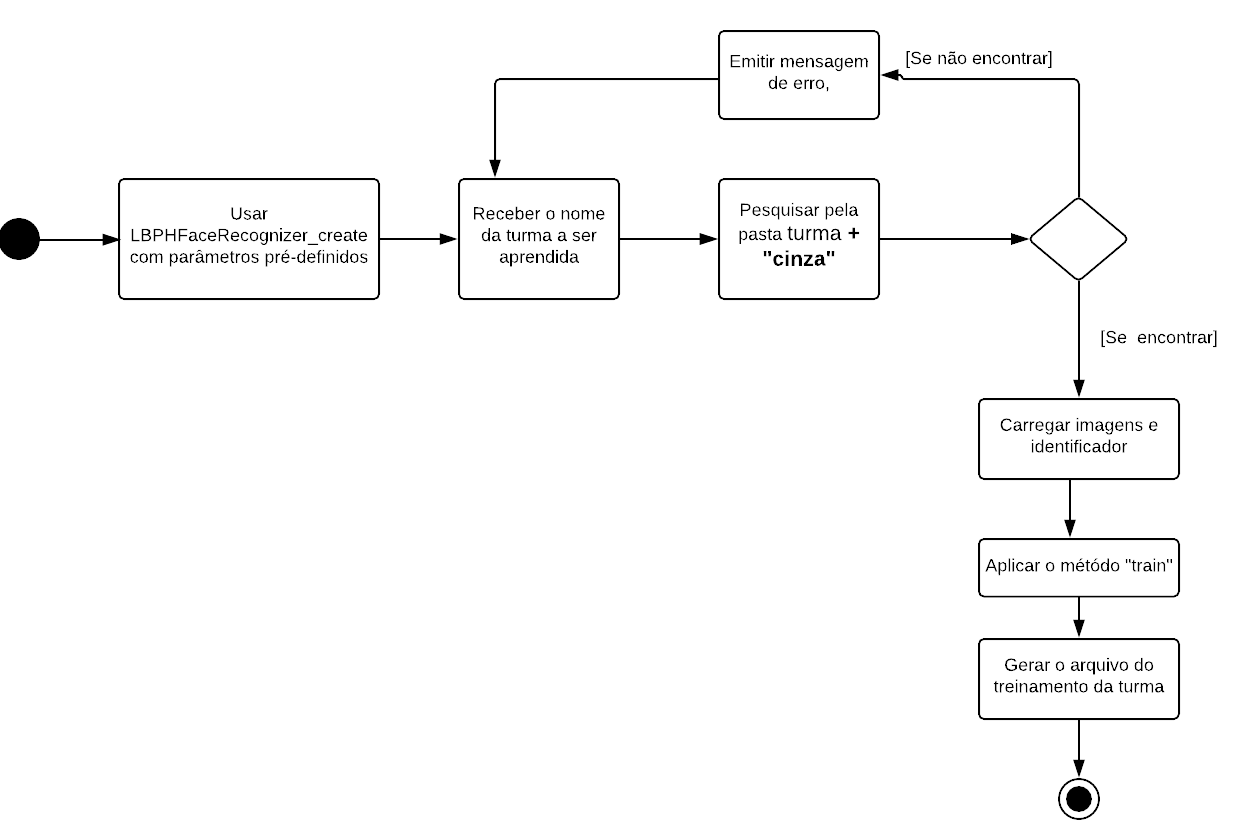
\includegraphics[width=1.0\textwidth]{diagramainteligencia.png}   
	\caption{Diagrama de atividades da fase treinamento}
	\label{fig:figura55}
\end{figure}

\section{O reconhecimento}
\noindent 
A etapa seguinte consiste em a partir de uma fotografia recebida da turma identificar quem nela encontra-se presente. Ela é realizada através do arquivo "reconhecimento\_final.py". 

Como mencionado no início do capítulo, inicialmente, ele procura por fotografias em uma pasta denominada "faltas". Quando detecta a presença de uma fotografia na pasta, inicia-se o processo. Do nome da foto, se extrai o nome da turma a qual ela pertence, a disciplina, o dia, mês e ano, o tempo de aula. A figura \ref{fig:figura56} mostra um exemplo com explicação dos campos, perceba que turma2 é o nome da turma e IA o nome da disciplina. A identificação da disciplina e do tempo de aula fazem-se necessárias, uma vez que uma disciplina pode durar  mais do que 1 tempo de aula. Assim, um aluno pode ter faltado ao 1º tempo, mas ter comparecido no 2º. 

\begin{figure}[!ht]
	\centering
	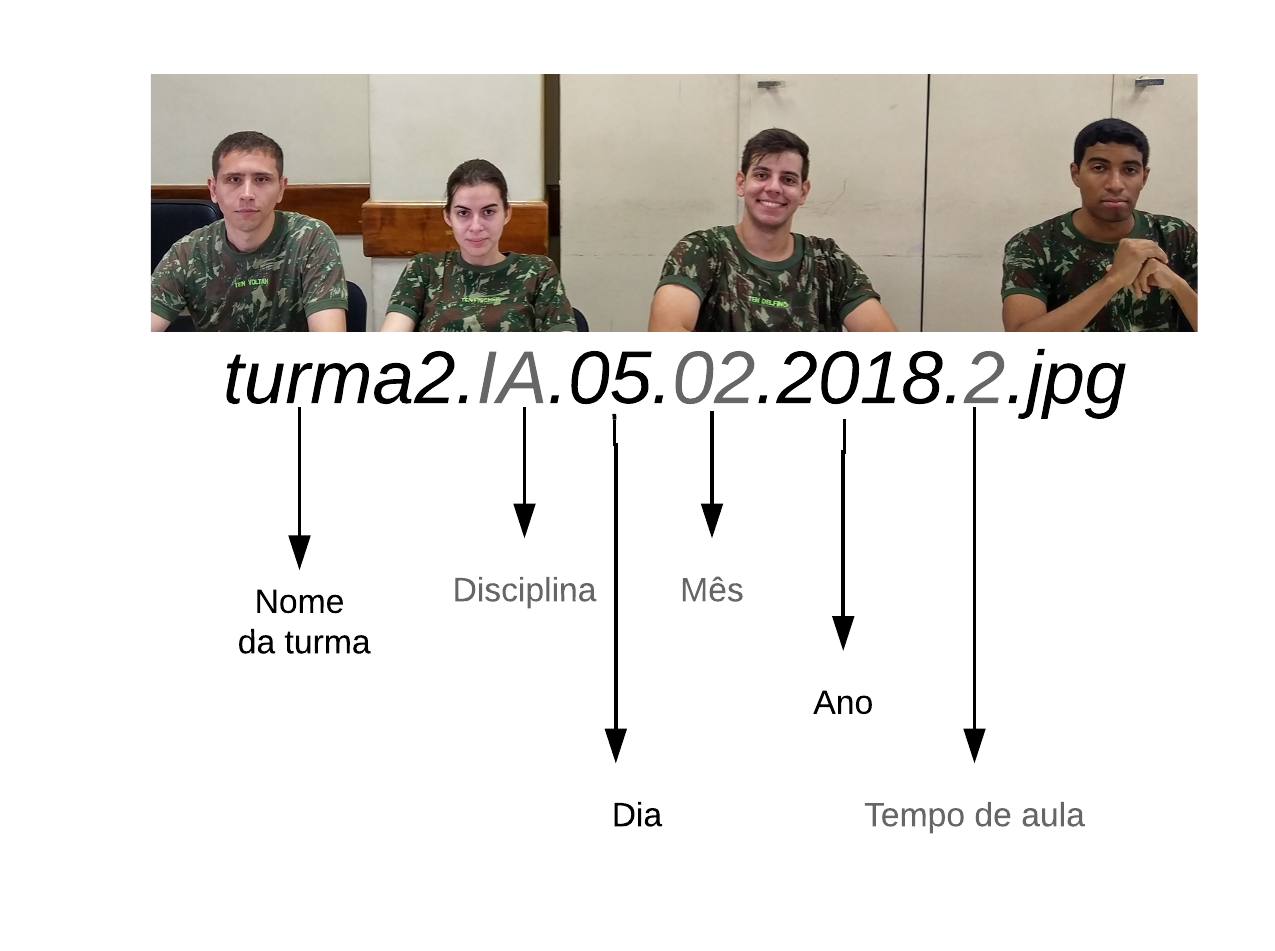
\includegraphics[width=0.7\textwidth]{nomenclaturaFotoTurma.png}   
	\caption{Exemplo de nome da foto}
	\label{fig:figura56}
\end{figure}

Ao encontrar uma imagem, ela é carregada, tratada, isso é, convertida para escala cinza, redimensionada e tem suas faces frontais detectadas. A partir do nome da turma, busca-se o arquivo que concatena as informações do banco de imagens daquela turma,  gerado na etapa treinamento. Tem-se aqui um ponto a ser destacado, o trabalho consiste em comparar características, usando o LBPH, daquela uma face com as faces previamente catalogadas para aquela turma. Como explicado, o algoritmo verifica a menor distância e depois compara com o\textit{threshold}. Cada uma das faces é reconhecida, ou no caso da menor distância ainda ser maior que o \textit{threshold}, ela é atribuída como desconhecida. O retorno do reconhecimento da face é o código do aluno. Aquele que teve sua face reconhecida tem sua presença computada. Em cada uma das faces detectadas, desenha-se o retângulo delimitador e a matrícula do aluno. Essas informações sobre composição de turma e o registro da presença serão realizadas utilizando-se o banco de dados, e serão abordadas com mais detalhes no capítulo 6, que tratará sobre o banco de dados.
%Em uma primeira fase desse projeto essas informações sobre composição de turma e presença estarão no próprio script em Python/saída. Na etapa futura, com a implementação do módulo BD, elas passarão a ser consultadas e salvas no próprio banco de dados.  

Após a imagem receber o retângulo com o nome do aluno, essas alterações são salvas e o arquivo migra para a pasta \textit{apuradas}. Ao nome da imagem, antes do formato, é feita a adição do caracter '.'  e o número daquela imagem, isso é, '.1' se for a primeira, '.2' se for a segunda e assim por diante. Por exemplo, caso a fotografia da figura \ref{fig:figura54} ao ser movida de pasta, verifique-se que foi a 5ª imagem apurada da turma2, na disciplina IA, no dia 05/02/2018 em seu 2º tempo de aula, então ao ser movido para a pasta apuradas, ela passaria a se chamar \textit{turma2.IA.05.02.2018.2.5.jpg}. 

A migração da imagem entre pastas garante que o laço \textit{while} não acabe tendo de verificar fotos que já foram apuradas. Além disso, a manutenção da imagem, em uma outra pasta, permite que caso algum aluno conteste  a falta, tenha-se um mecanismo alternativo para verificar essa informação. Nesse caso, a imagem da turma poderia ser utilizada, como mecanismo de verificação secundário. A figura \ref{fig:figura57} ilustra um diagrama de atividades para o "reconhecimento\_final.py". Nele, é possível verificar que o servidor procura pela fotografia na pasta faltas, quando encontra inicia seu processo de reconhecimento, e ao final transfere a fotografia apurada (com as faces identificadas por um retângulo branco com a matricula do aluno) para a pasta apuradas. Dessa forma ele está sempre verificando a pasta faltas.
   
\begin{figure}[!ht]
	\centering
	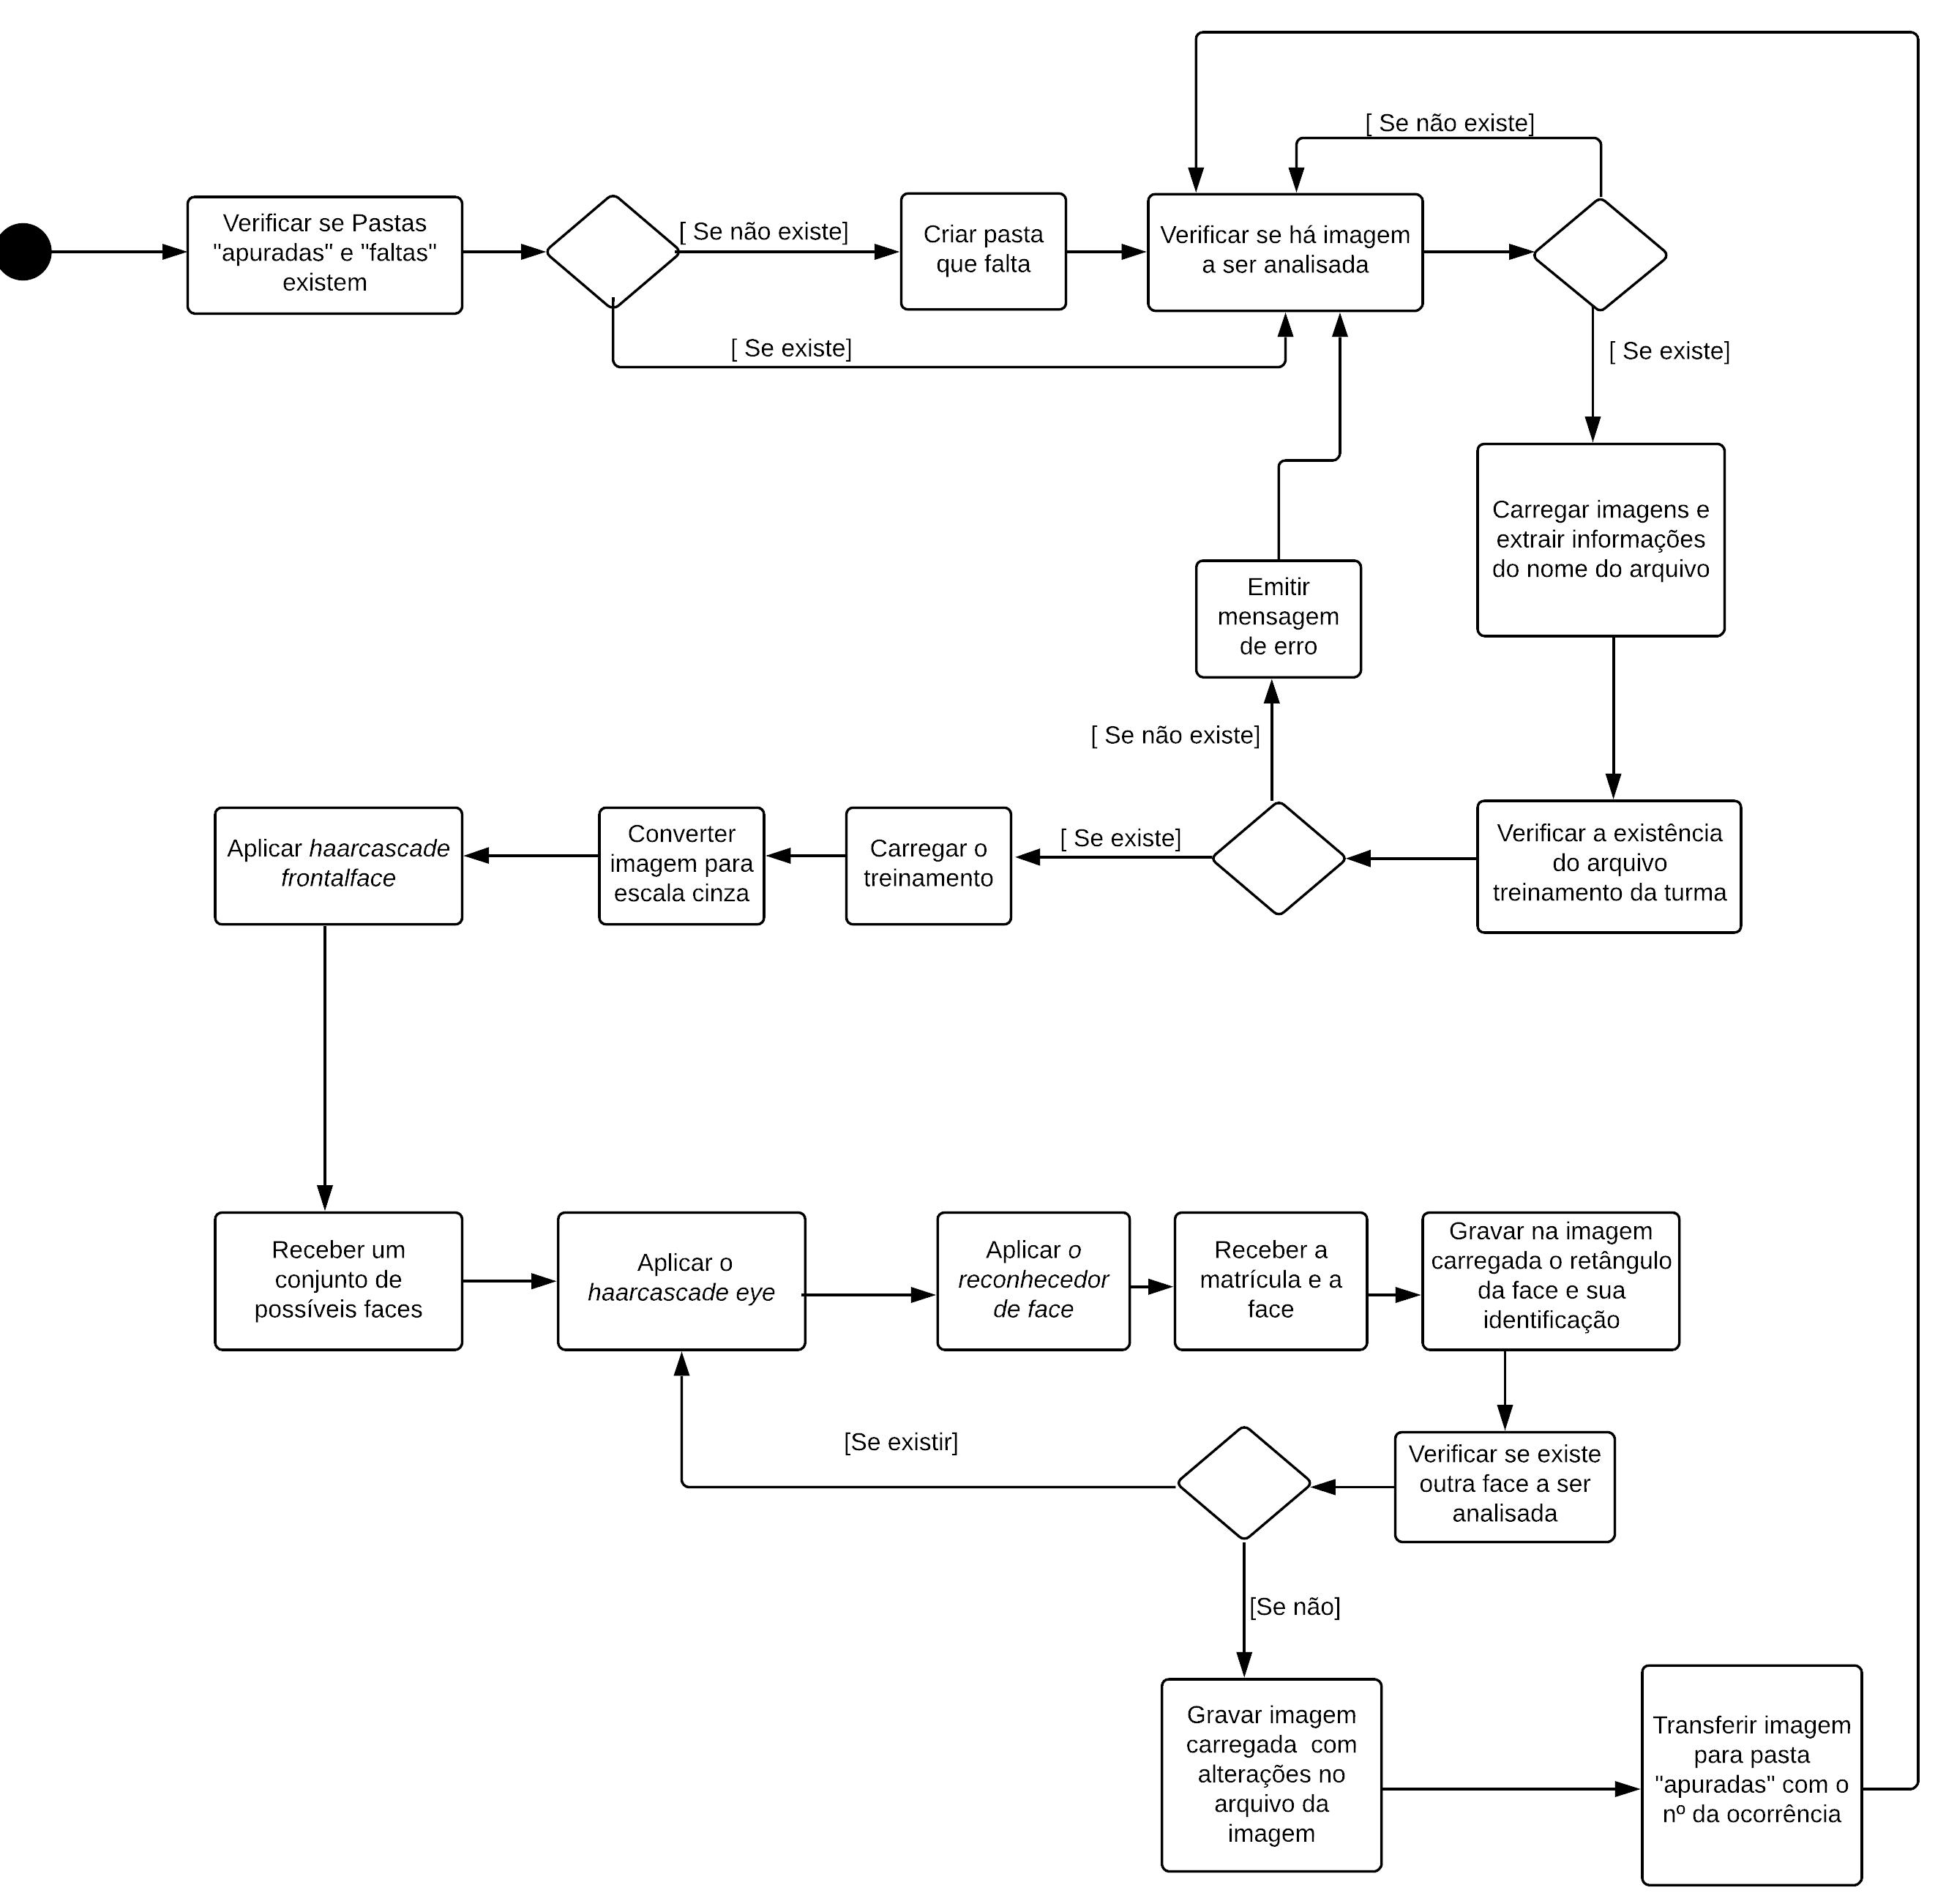
\includegraphics[width=1.0\textwidth]{diagramarec.png}   
	\caption{Diagrama de atividades da fase reconhecimento}
	\label{fig:figura57}
\end{figure}

A figura \ref{fig:figura58} ilustra em \textit{a)} a imagem de entrada do módulo Servidor, ou seja, a  recebida, e em \textit{b)} a imagem de saída, ou seja, a que será salva na pasta \textit{apuradas}. Comparando \textit{a)} e \textit{b)}, pode-se perceber que  adicionou-se o retângulo na face acompanhado da matrícula do aluno. Dessa forma atende-se o requisito funcional \textit{RF04 - Armazenar fotografia}.

\begin{figure}[!ht]
	\centering
	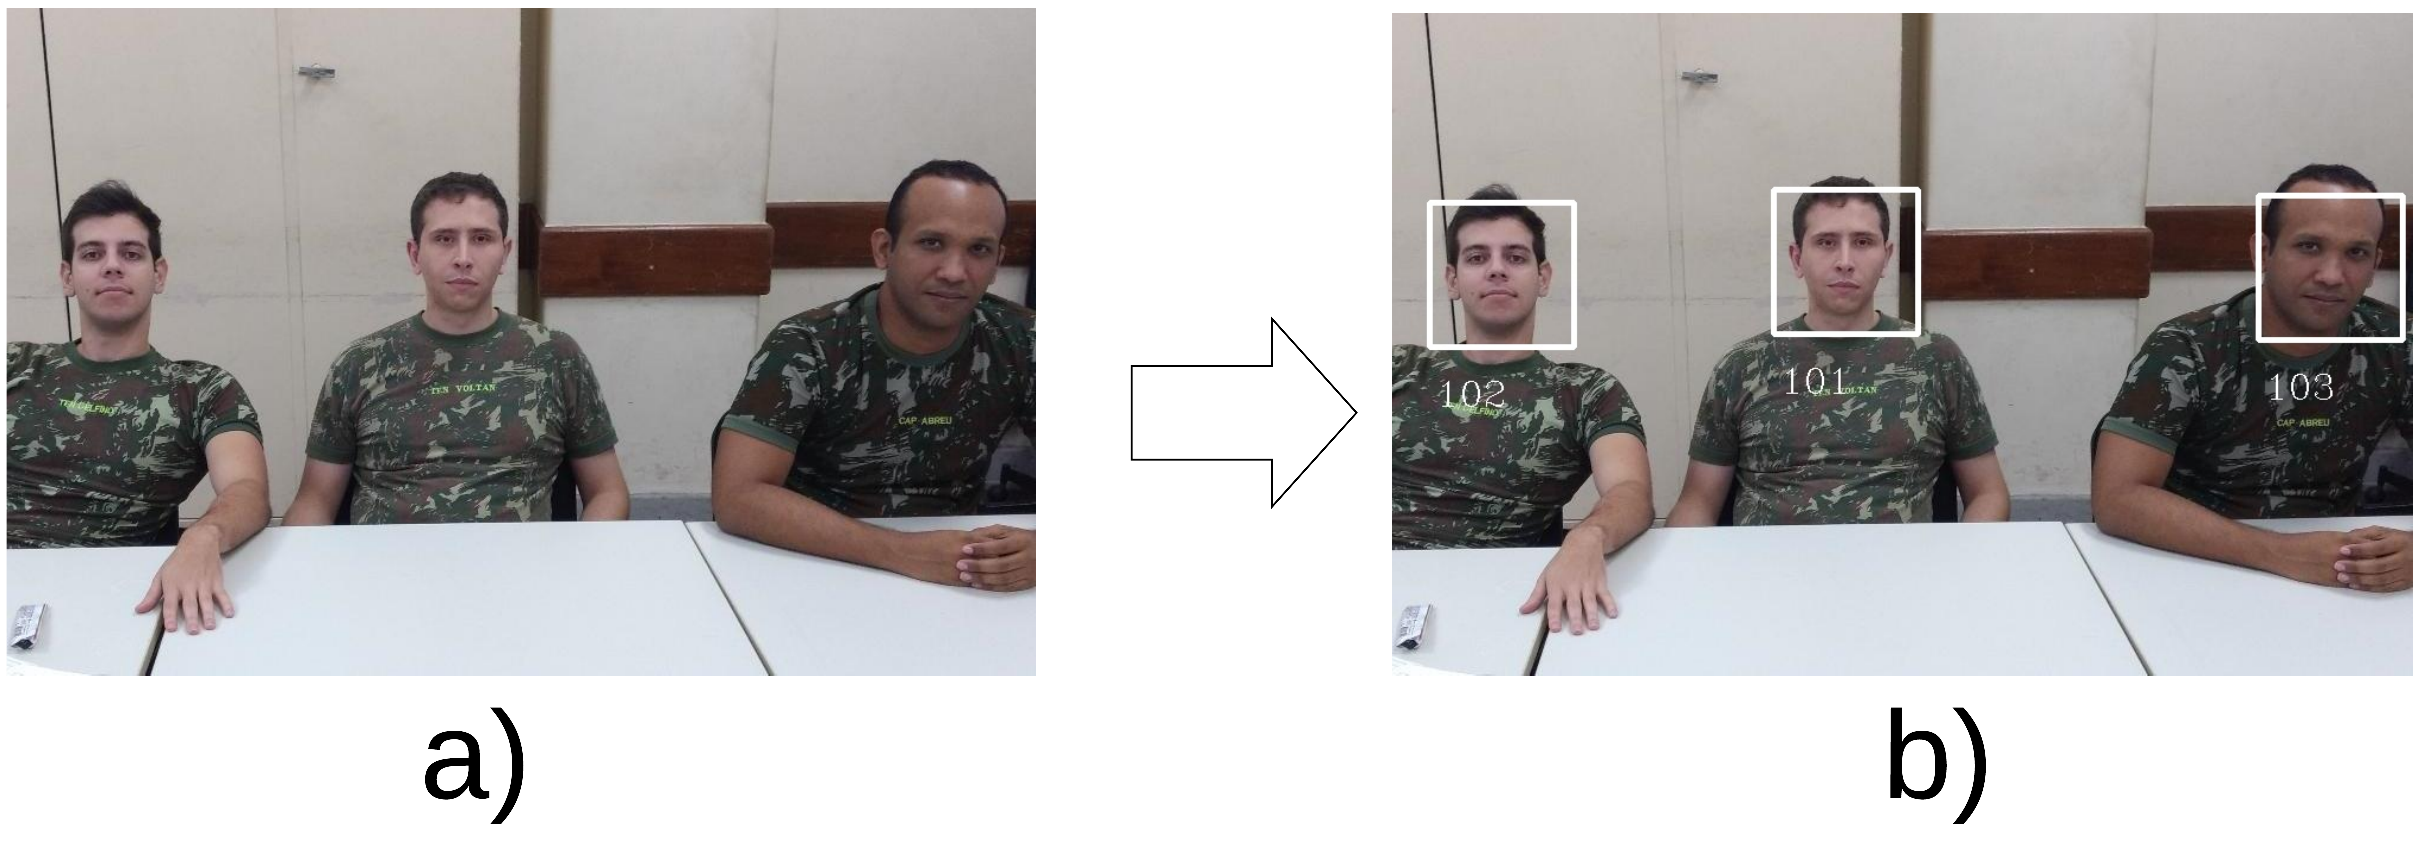
\includegraphics[width=1.0\textwidth]{antesdepoisbranco.png}   
	\caption{Entrada e saída do módulo Servidor}
	\label{fig:figura58}
\end{figure}
